% Name: Heat map
% Description: A grid of values colored by size, with each value printed in its cell.
% Tags: heat map, matrix plot, colormap

\usepackage{pgfplots}
\pgfplotsset{compat=1.18}

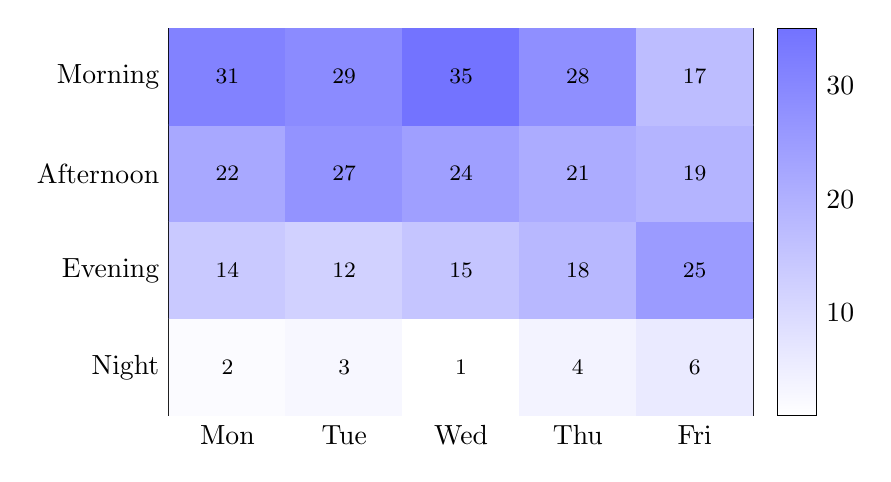
\begin{tikzpicture}
  \begin{axis}[
    width=9cm, height=6.5cm, enlargelimits=false,
    colormap={blues}{color=(white) color=(blue!55)}, colorbar,
    xtick={0,...,4}, xticklabels={Mon, Tue, Wed, Thu, Fri},
    ytick={0,...,3}, yticklabels={Night, Evening, Afternoon, Morning},
    tick style={draw=none},
    nodes near coords={\pgfmathprintnumber\pgfplotspointmeta},
    nodes near coords style={font=\footnotesize, anchor=center},
  ]
    \addplot[matrix plot*, mesh/cols=5, point meta=explicit] coordinates {
      (0,0) [2]  (1,0) [3]  (2,0) [1]  (3,0) [4]  (4,0) [6]

      (0,1) [14] (1,1) [12] (2,1) [15] (3,1) [18] (4,1) [25]

      (0,2) [22] (1,2) [27] (2,2) [24] (3,2) [21] (4,2) [19]

      (0,3) [31] (1,3) [29] (2,3) [35] (3,3) [28] (4,3) [17]
    };
  \end{axis}
\end{tikzpicture}
